\documentclass{beamer}

% For more themes, color themes and font themes, see:
% http://deic.uab.es/~iblanes/beamer_gallery/index_by_theme.html
%
\mode<presentation>
{
	\usetheme{Warsaw}       % or try default, Darmstadt, Warsaw, ...
	\usecolortheme{default} % or try albatross, beaver, crane, ...
	\usefonttheme{serif}    % or try default, structurebold, ...
	\setbeamertemplate{navigation symbols}{}
	\setbeamertemplate{caption}[numbered]
} 

\usepackage[english, russian]{babel}
\usepackage[utf8x]{inputenc}
\usepackage{chemfig}
\usepackage[version=3]{mhchem}

% On Overleaf, these lines give you sharper preview images.
% You might want to `comment them out before you export, though.
\usepackage{pgfpages}
\pgfpagesuselayout{resize to}[%
physical paper width=8in, physical paper height=6in]
% slide numbering
\setbeamertemplate{page number in head/foot}[totalframenumber]

\newtheorem{cor}{Следствие}
\newtheorem{theor}{Теорема}
\newtheorem{defin}{Определение}
\newtheorem{case}{Случай}
\AtBeginEnvironment{case}{%
    \setbeamercolor{block title}{use=example text,fg=white,bg=orange!70!white}
	\setbeamercolor{block body}{parent=normal text,fg=black, bg=orange!30!white}
}
\newtheorem{probl}{Гипотеза}
\newtheorem{exampl}{Пример}
\AtBeginEnvironment{exampl}{%
	\setbeamercolor{block title}{use=example text,fg=white,bg=example text.fg!75!black}
	\setbeamercolor{block body}{parent=normal text,use=block title example,bg=block title example.bg!10!bg}
}

\title[]{Условные нижние оценки для задачи поиска путей с контекстно-свободными ограничениями}
\author[Истомина Александра (СПбГУ)]{Истомина Александра \\ \vspace{1cm}
\small{Научный руководитель: Григорьев Семён Вячеславович}}
\institute{Санкт-Петербургский государственный университет}
\date{16 июня 2023 г.}

\begin{document}
	
\begin{frame}
	\titlepage
\end{frame}

\begin{frame}{Определения}
	\textit{Контекстно-свободная грамматика} --- это четверка $G=(N, \Sigma, P, S)$, где:
	
	\begin{itemize}
		\item $N$ --- конечное множество нетерминалов
		\item $\Sigma$ --- конечный алфавит
		\item $P$ --- конечное множество правил вывода
		\item $S \in N$ --- стартовый нетерминал
	\end{itemize}

	\textit{Шаг вывода} --- это операция $\alpha A \beta \Rightarrow \alpha \gamma \beta$, где $\alpha, \gamma, \beta \in (\Sigma \cup N)^*$, а $A \rightarrow \gamma \in P$. 
	
	$\mathcal{L}(G) = \{w \in \Sigma^*| S \Rightarrow \ldots \Rightarrow w\}$ --- язык, задаваемый грамматикой.
	
	\begin{exampl}[Язык Дика на $k$ типах скобок, Dyck-$k$]
		\begin{itemize}
			\item $N = \{S\}$
			\item $\Sigma = \{(_i, )_i\}, \forall i = 1, \ldots, k$
			\item Правила вывода: $S \rightarrow \epsilon | SS | (_1 S )_1 | \ldots | (_k S )_k$, где $\epsilon$ --- это пустая строка. 
		\end{itemize}
	\end{exampl}
\end{frame}

\begin{frame}{Определения}
	\begin{defin}[Задача контекстно-свободной достижимости, CFL reachability]
		\textbf{Дано:} ориентированный граф $D = (V, E, L)$ с пометками на ребрах $L \subseteq \Sigma$, КС грамматика $G = (N, \Sigma, P, S)$.
		
		\textbf{Надо:} понять, есть ли путь между вершинами, такой что пометки на ребрах образуют слово из $\mathcal{L}(G)$.
		
		Варианты: all-pairs/s-t
	\end{defin}

	Грамматика обычно предполагается фиксированной. Сложность алгоритма считается от $n = |V|$ --- количества вершин в графе.
\end{frame}
	
\begin{frame}{История}
	Известныe алгоритмы: 
	\begin{center}
		\begin{itemize}
			\item[] [Melski, Reps 1997] $\mathcal{O}(n^3)$
			\item[] [Chaudhuri 2008] $\mathcal{O}(n^3 / \log n)$
		\end{itemize}
	\end{center}
	\textbf{Вопрос:} Существует ли алгоритм со временем работы $\mathcal{O}(n^{3-\epsilon}), \epsilon > 0$?
	
	\vspace{1cm}
	Способы решения:
	
	\begin{itemize}
		\item Придумать более быстрый алгоритм
		\item Найти нижнюю оценку на сложность
	\end{itemize}
\end{frame}


\begin{frame}{Условные нижние оценки}
	\textit{Условная нижняя оценка} --- верна, если верна некоторая гипотеза
	
	Получаются с помощью сведений от одной задаче к другой. 
	
	\vspace{1cm}
	
	\textit{Сведение} (A, $t_A$) $\rightarrow$ (B, $t_B$):
	
	\begin{center}
		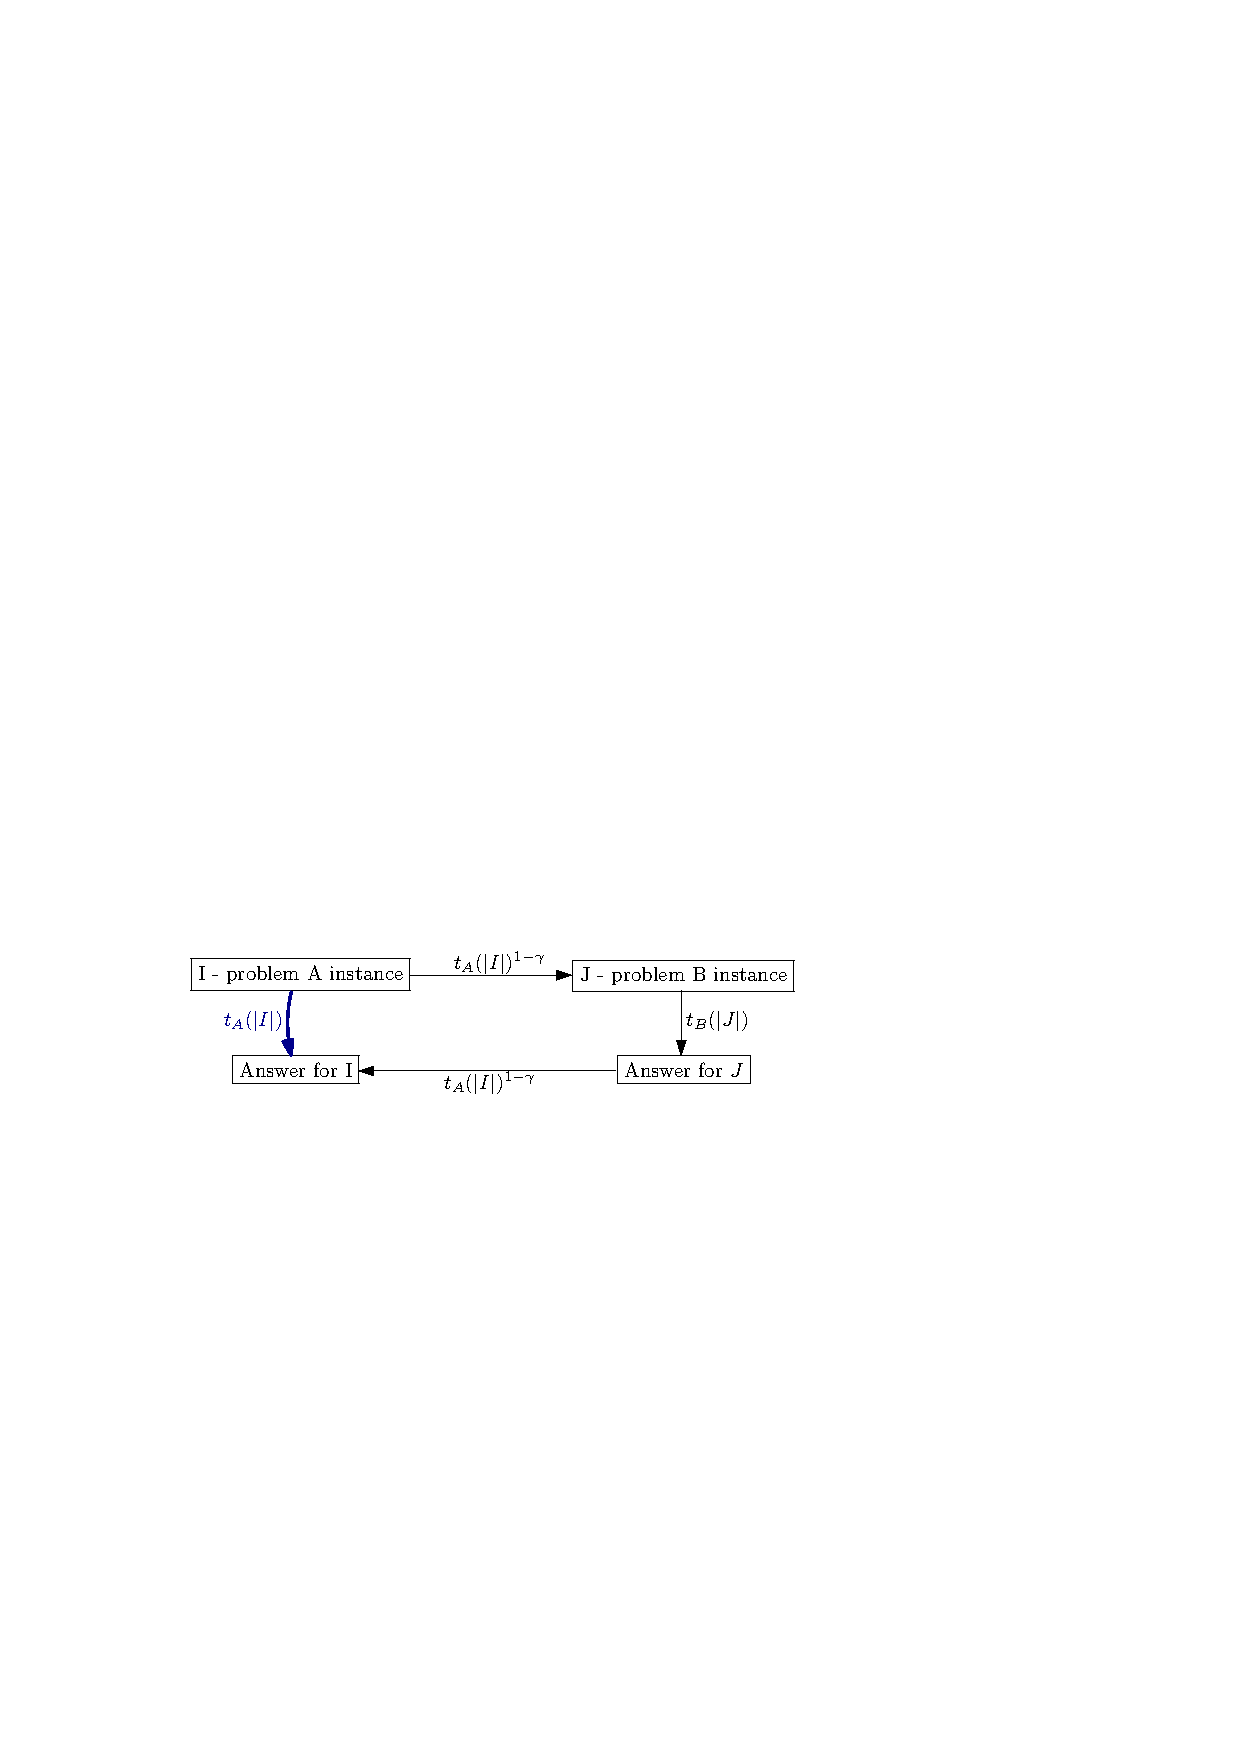
\includegraphics[scale=0.85]{./pictures/reduction.pdf}
	\end{center}

	Цель: найти задачу $X$ с гипотезой об ее временной сложности и свести ее к задаче CFL reachability. 
\end{frame}


\begin{frame}{Популярные задачи и гипотезы}
		
	\begin{probl}[BMM]
		Перемножить две булевы матрицы размера $n \times n$ нельзя комбинаторным алгоритмом за время $\mathcal{O}(n^{3 - \epsilon}), \epsilon > 0$.
	\end{probl}

	\begin{probl}[SAT]
		(N)SETH - определить выполнимость булевой формулы нельзя (ко-недетерминированно) за время $\mathcal{O}(2^{(1 - \epsilon)n}), \epsilon > 0$.
	\end{probl}
	
	\begin{probl}[APSP]
		Найти наименьшие расстояния между всеми парами вершин во взвешенном графе нельзя за время $\mathcal{O}(n^{3 - \epsilon}), \epsilon > 0$.	\end{probl}

	\begin{probl}[3SUM]
		Определить, есть ли в массиве тройка чисел, суммирующаяся в 0, нельзя за время $\mathcal{O}(n^{2 - \epsilon}), \epsilon > 0$.
	\end{probl}
\end{frame}

\begin{frame}{Карта сведений}
	\begin{center}
		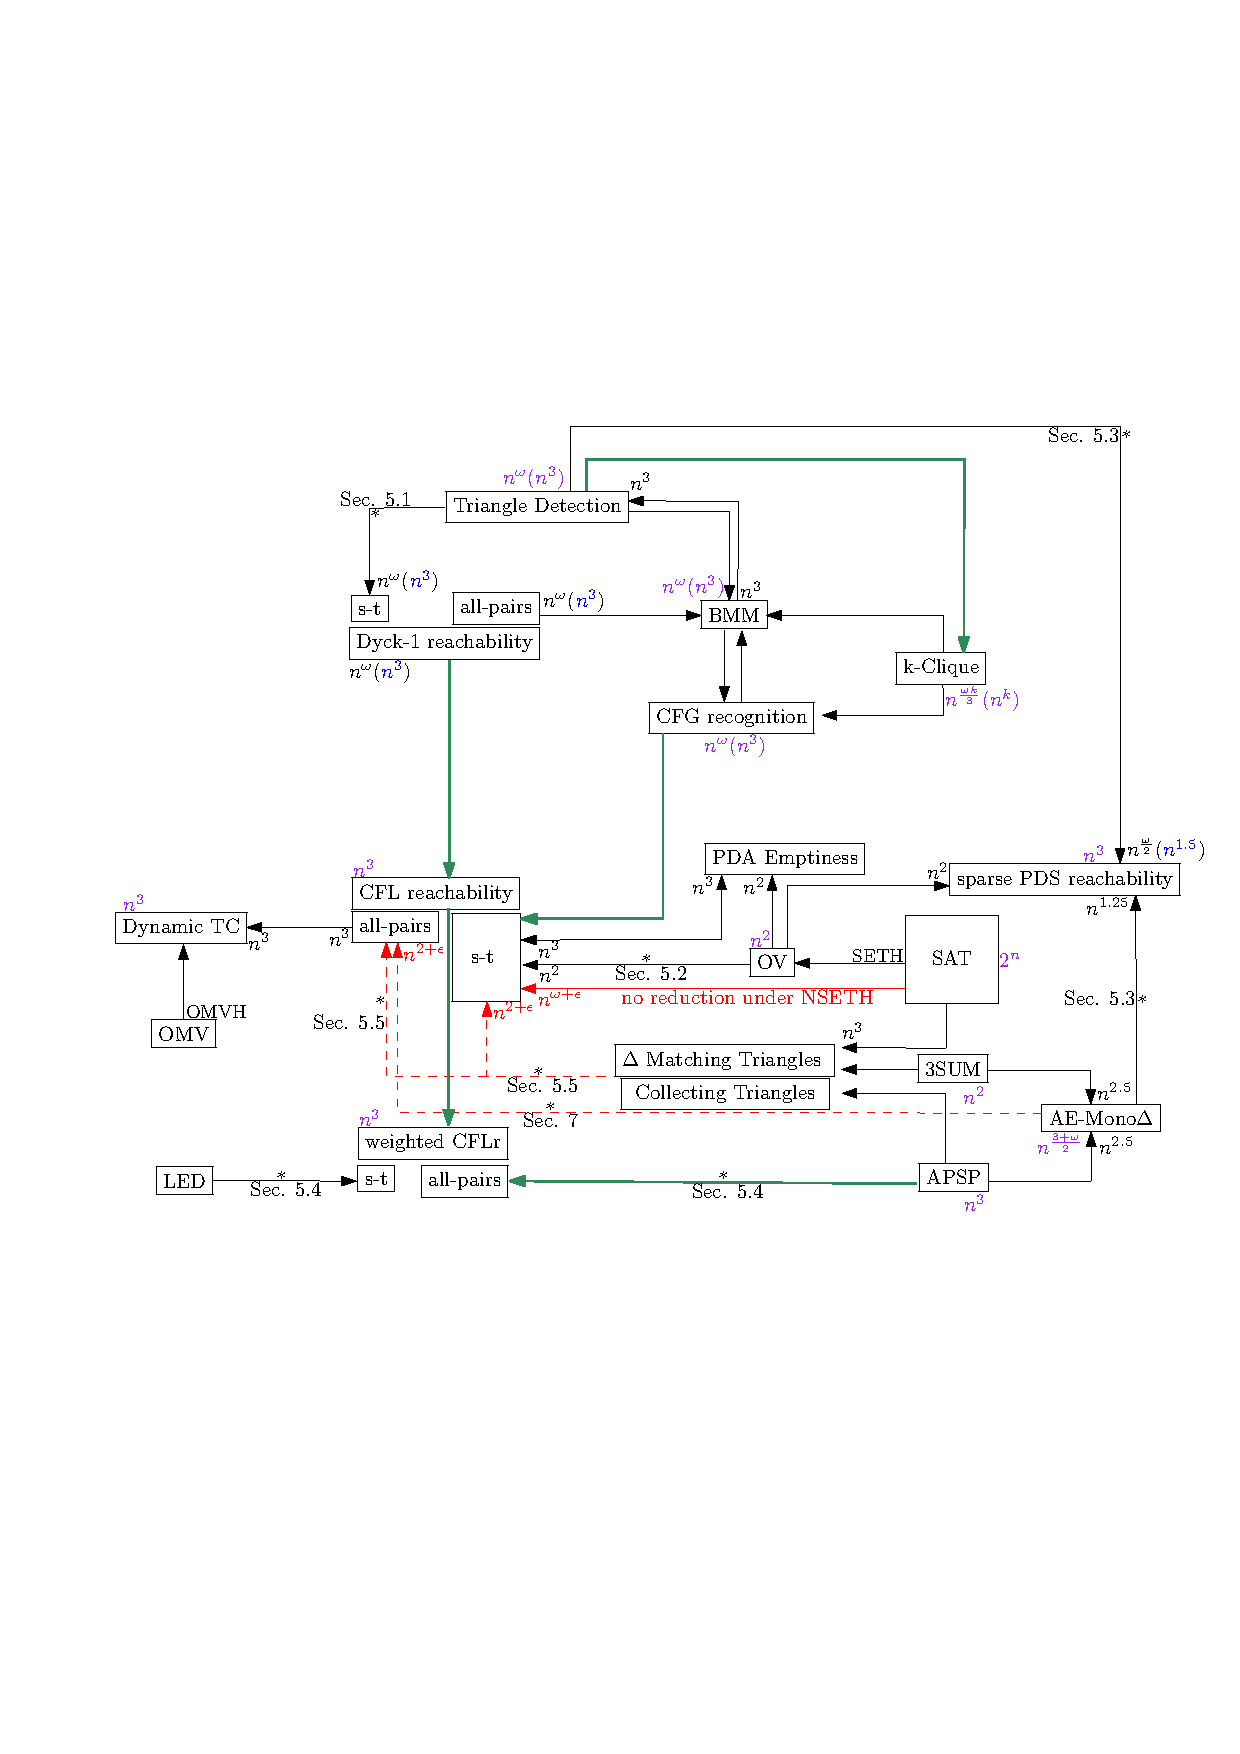
\includegraphics[scale=0.58]{./pictures/map_popl_m.pdf}
		%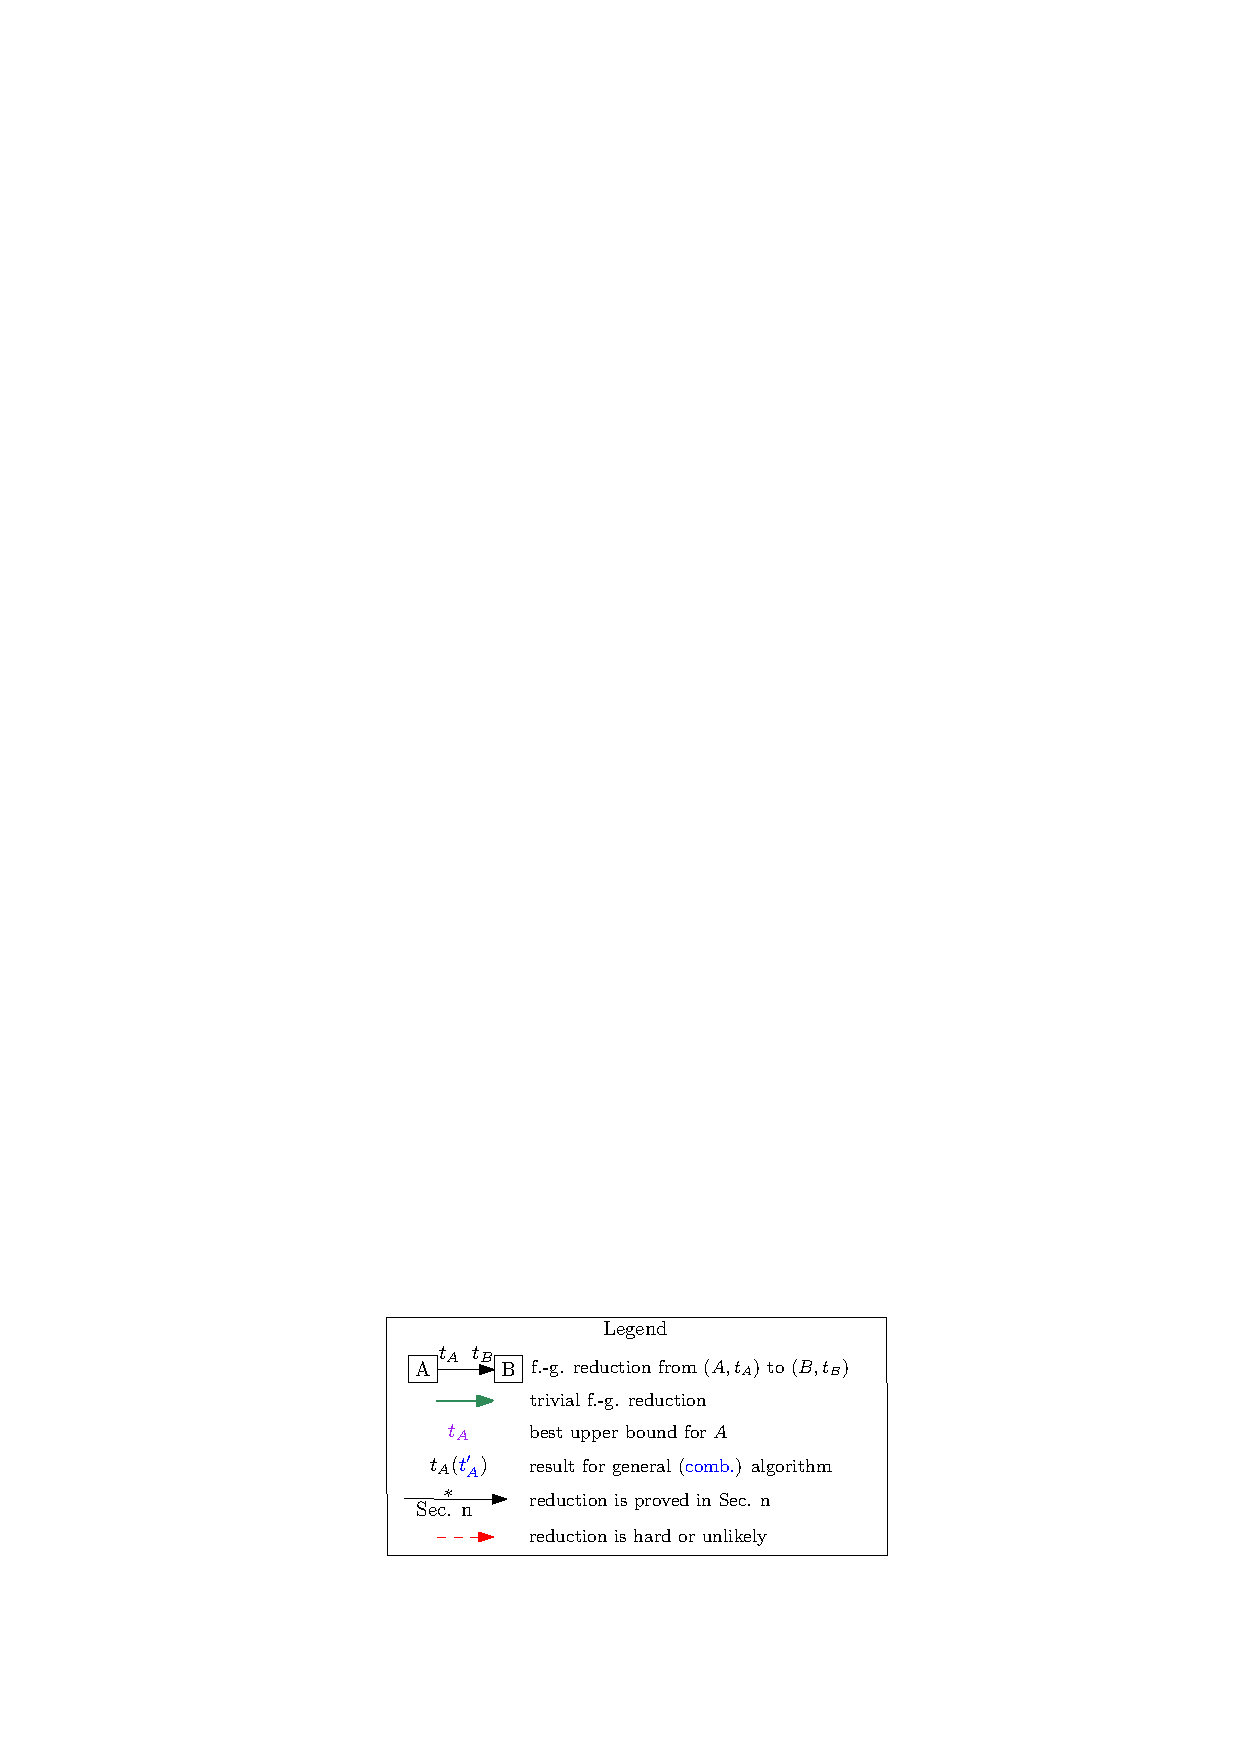
\includegraphics[scale=0.45]{./pictures/map_popl_l.pdf}
	\end{center}
\end{frame}
	
\begin{frame}{Результаты: Сведения}
	\begin{itemize}
		\item (Triangle Detection, $n^{\omega}$) $\rightarrow$ (Dyck-1 reachability,  $n^{\omega}$)
		
		\begin{center}
			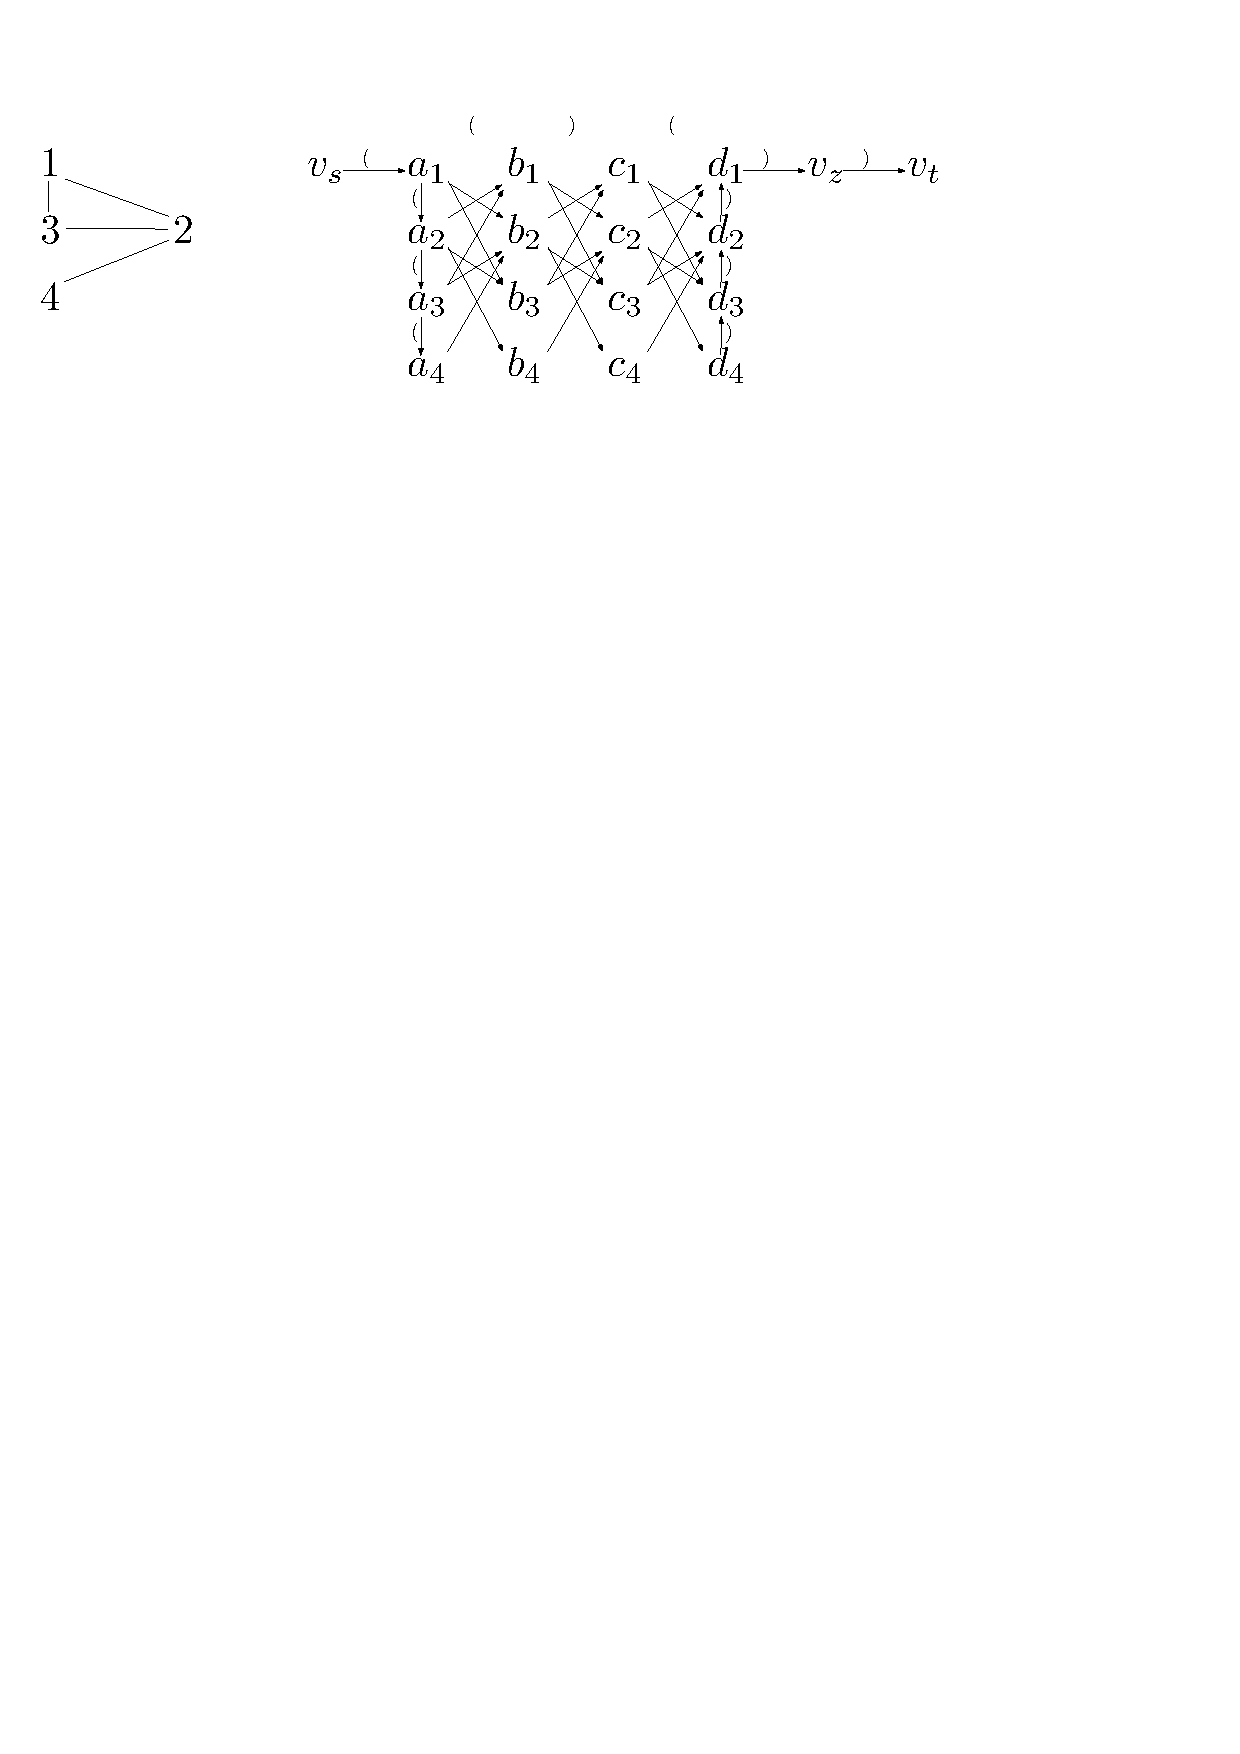
\includegraphics[scale=0.5]{./pictures/triangle_detection_example.pdf}
		\end{center}
		
		\item (OV, $n^{2}$) $\rightarrow$ (s-t CFL reachability,  $n^{2}$)
		
		\begin{center}
			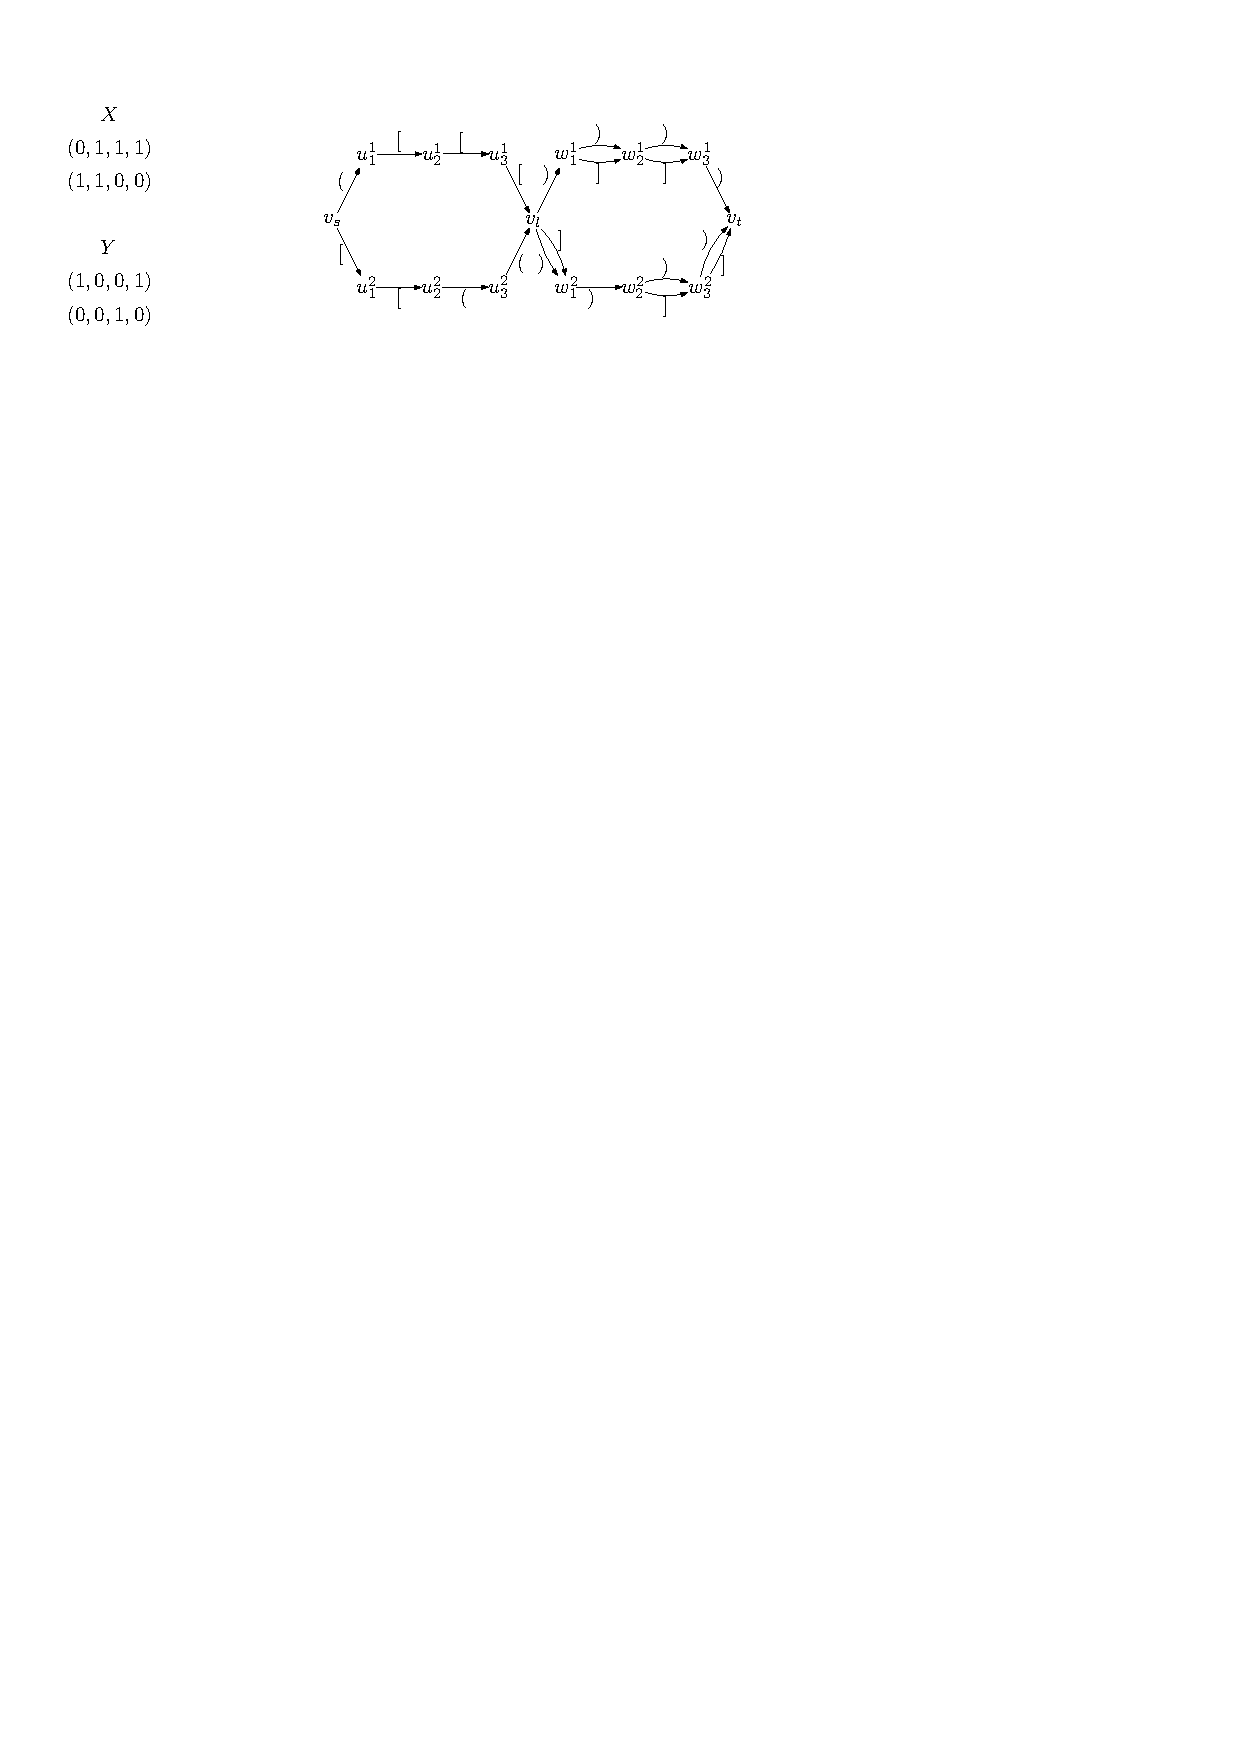
\includegraphics[scale=0.8]{./pictures/ov_to_cflr.pdf}
		\end{center}
	\end{itemize}
\end{frame}

\begin{frame}{Результаты: Сведения}
	\begin{itemize}
		\item (Triangle Detection, $n^{3}$) $\rightarrow$ (sparse PDS reachability with stack bound $\lceil \log n \rceil$,  $n^{1.5}$)
		
		\begin{center}
			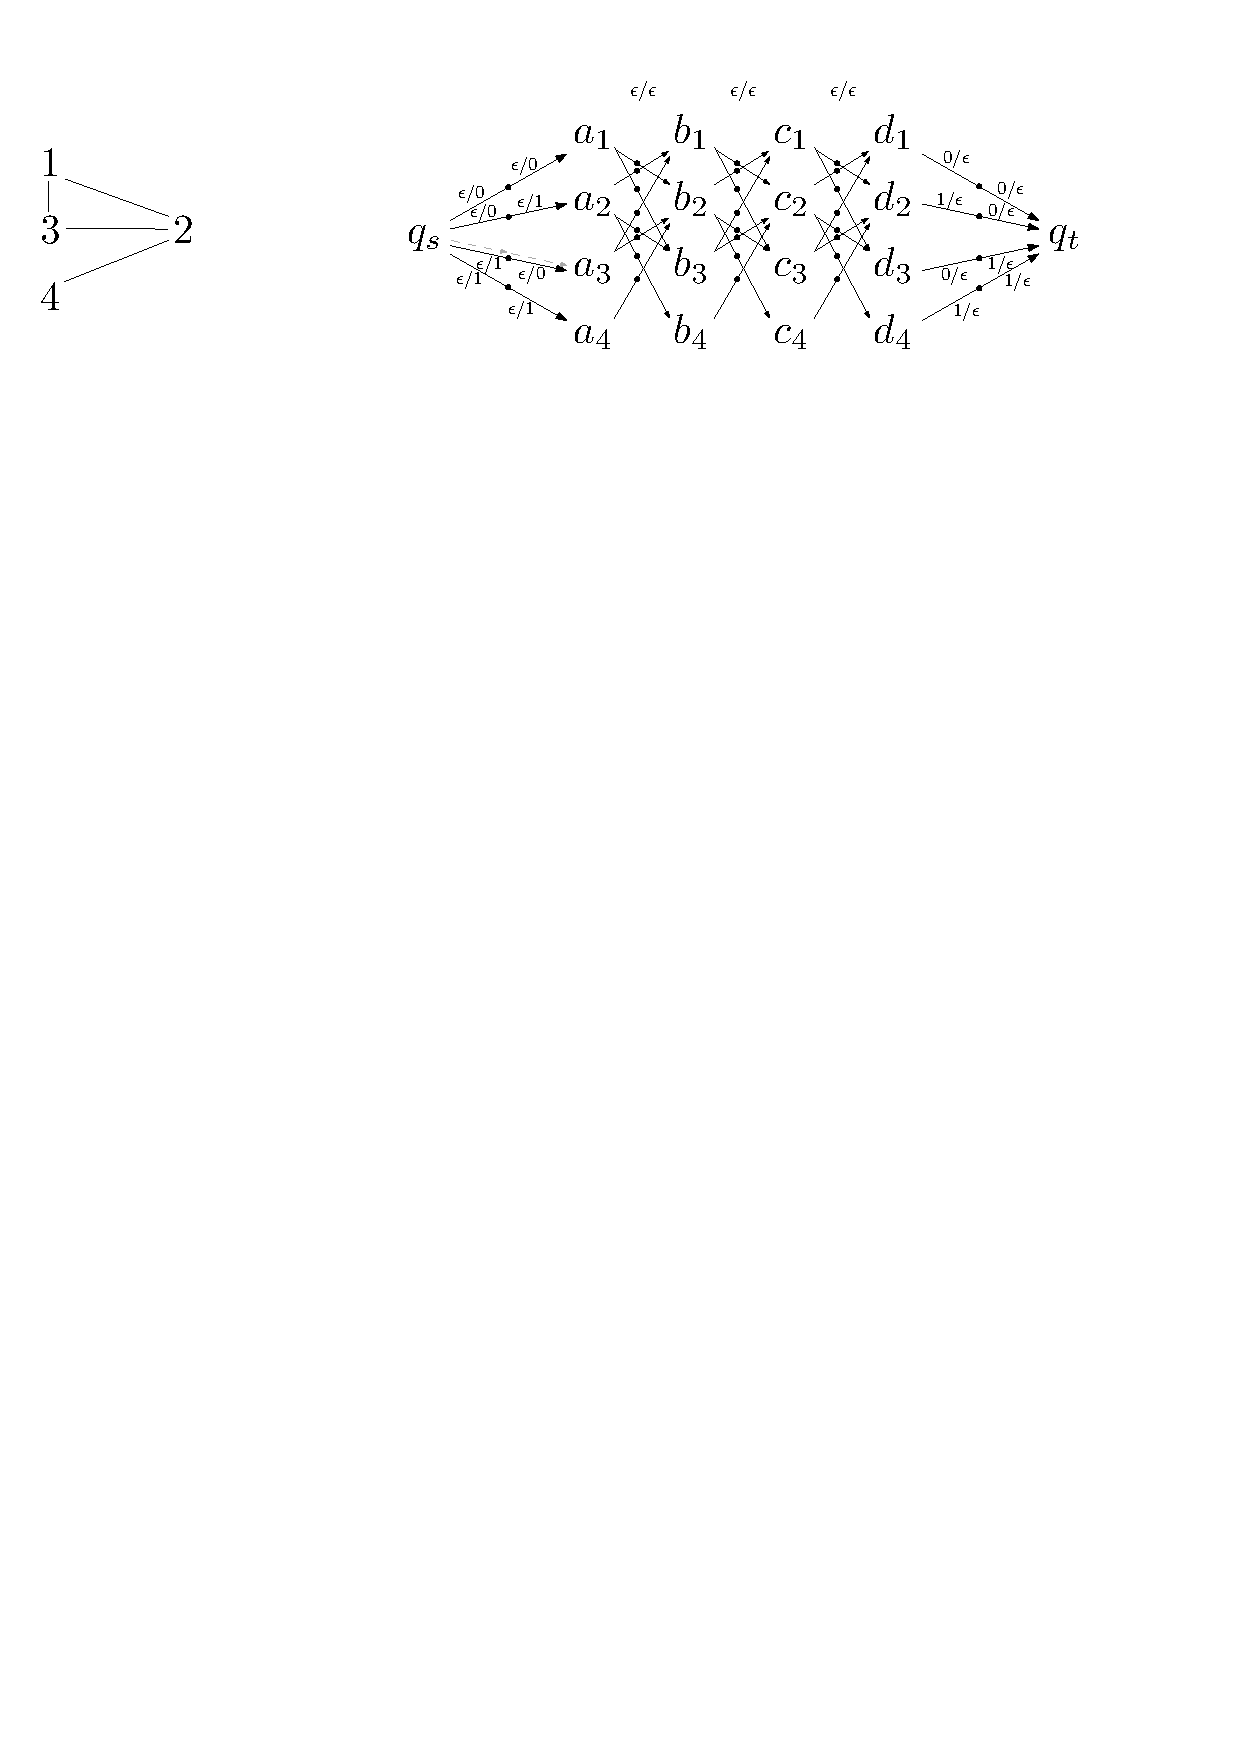
\includegraphics[scale=0.5]{./pictures/triangle_to_pds.pdf}
		\end{center}
		
		\item (AE-Mono$\Delta$, $n^{2.5}$) $\rightarrow$ (sparse PDS reachability with stack bound $4\lceil \log n \rceil$,  $n^{1.25}$)
		
		\begin{center}
			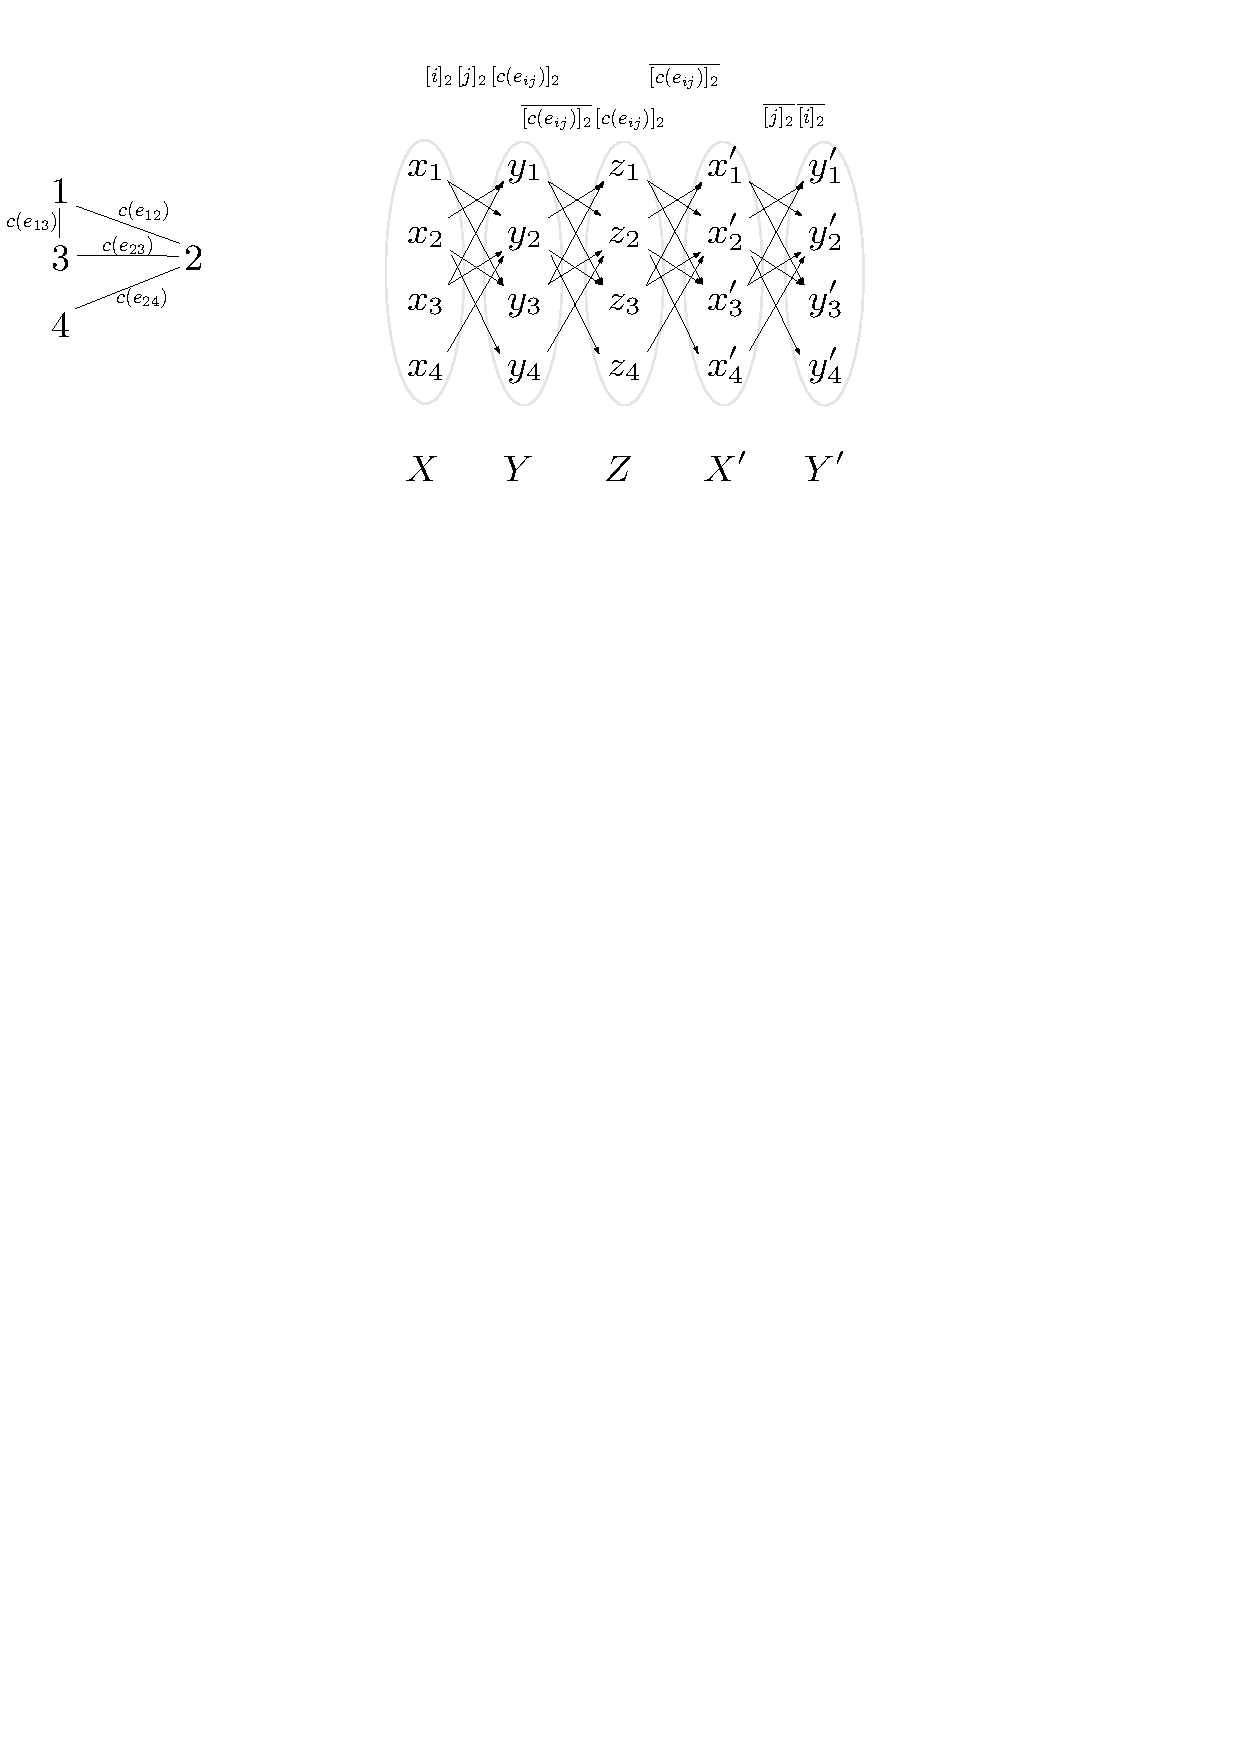
\includegraphics[scale=0.65]{./pictures/ae-monotr_to_cflr.pdf}
		\end{center}
	\end{itemize}
\end{frame}

\begin{frame}{Результаты: Сведения}
	\begin{itemize}
		\item (LED, $n^{c}$) $\rightarrow$ (weighted s-t CFL reachability,  $n^{c}$), $c > 1$
		
		\begin{center}
			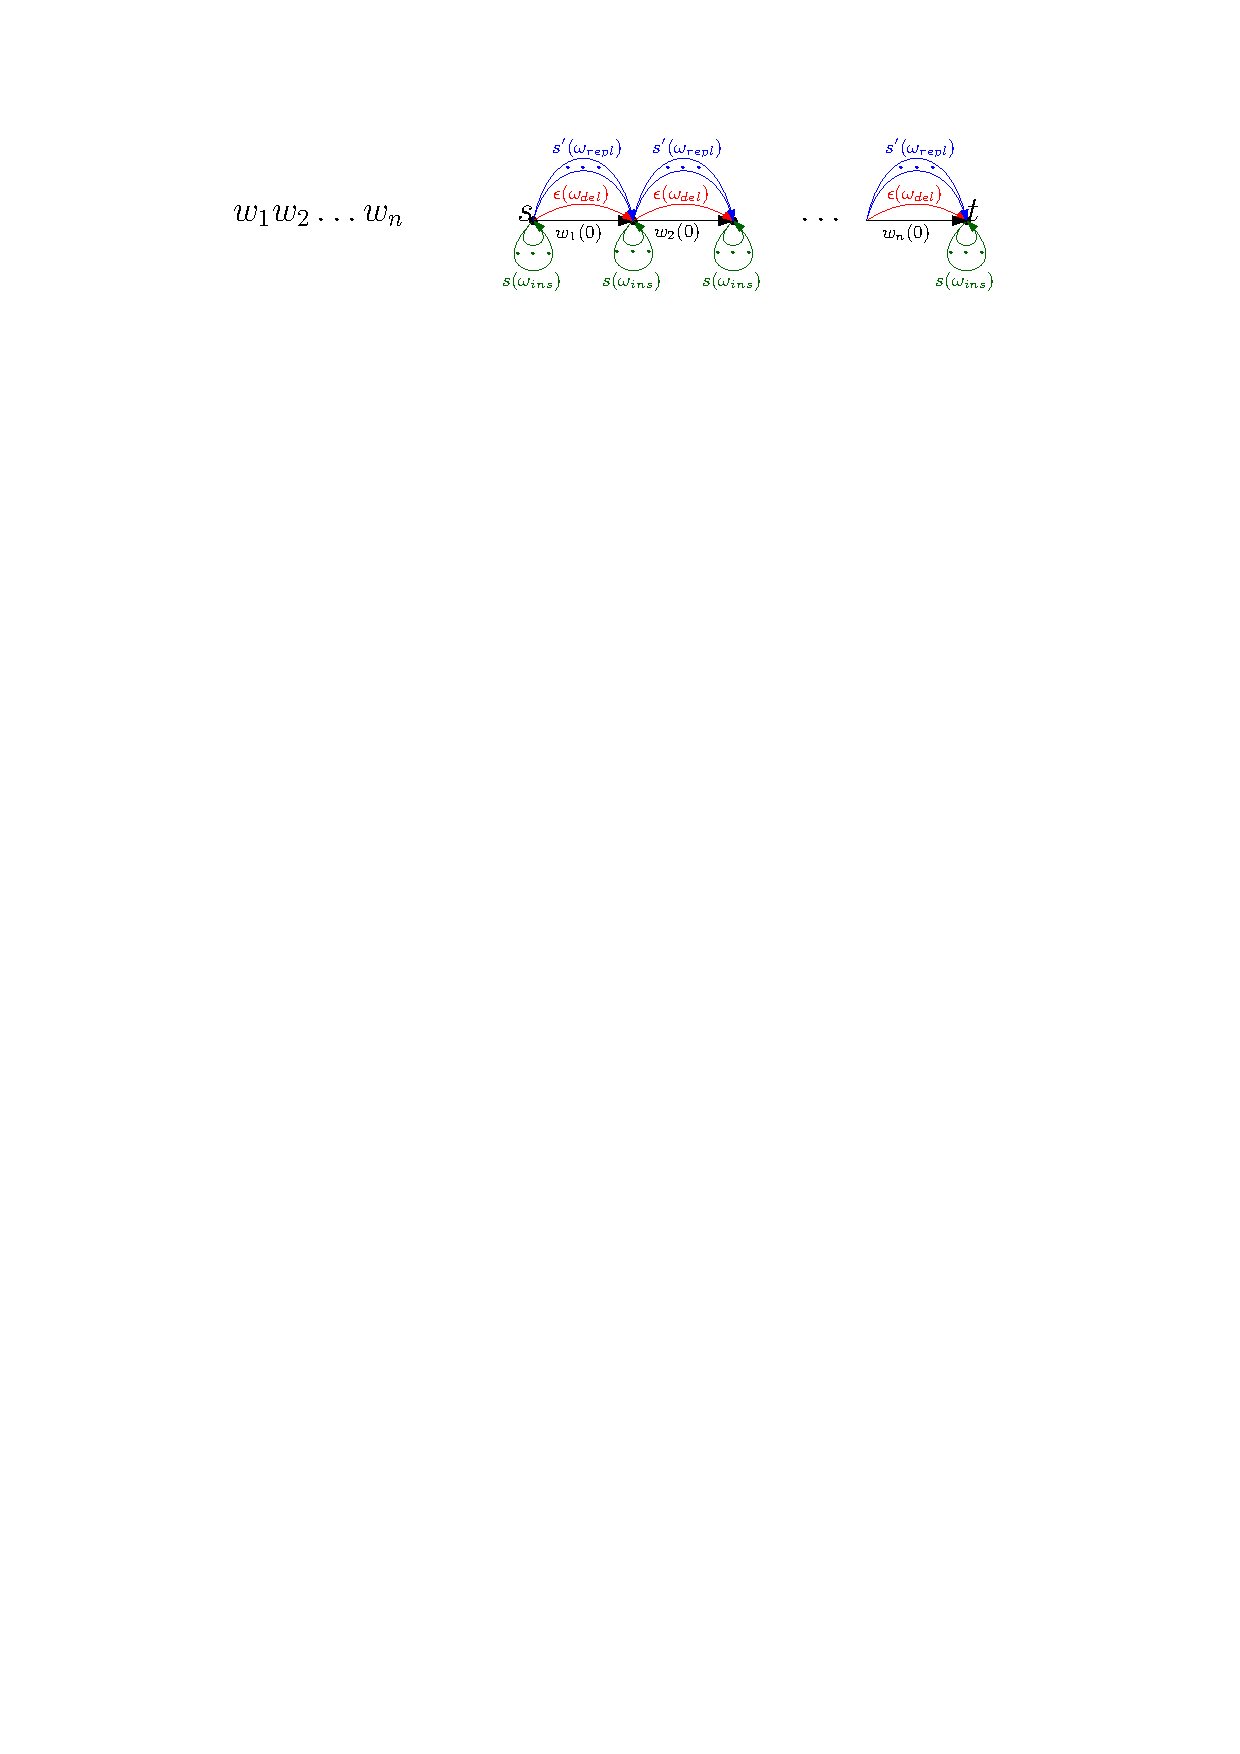
\includegraphics[scale=0.75]{./pictures/led_to_cflr.pdf}
		\end{center}
		
		\begin{cor}
			Для задачи weighted s-t CFL reachability не существует алгоритма со временем работы $\mathcal{O}(n^{3-\epsilon}), \epsilon > 0$, если APSP гипотеза верна.
		\end{cor}
	\end{itemize}
\end{frame}
	
	
\begin{frame}{Результаты: Потенциальные сведения}
	\begin{theor}
		Если существует сведение (Collecting Triangles/$\Delta$ Matching Triangles, $n^3$) $\rightarrow$ (CFL reachability, $n^c$), $c > 2$, то опровергается хотя бы одно из следующих утверждений:
		
		\begin{itemize}
			\item $\omega = 2$
			\item NSETH
			\item Cуществует сведение (all-pairs CFL reachability, $n^c$) $\rightarrow$ (s-t CFL reachability, $n^{c′} $), $c′ > 2$.
		\end{itemize}
	\end{theor}
\end{frame}


\begin{frame}{Результаты: Ограниченные пути}
	\begin{theor}[Schepper, 2018]
		Существует алгоритм для задачи s-t CFL reachability на ациклических графах со временем работы $\mathcal{O}(n^{\omega})$.
	\end{theor}

	\begin{cor}
		Существует алгоритм для задачи all-pairs CFL reachability на ациклических графах со временем работы $\mathcal{O}(n^{\omega})$.
	\end{cor}

	\begin{cor}
		Существует алгоритм для задачи all-pairs CFL reachability со временем работы $\tilde{\mathcal{O}}(n^c), c < 3$, находящий все $\mathcal{L}$-пути длины не более чем $k = \tilde{\mathcal{O}}(n^{c'})$, где $c' < \frac{3}{\omega} - 1$.
	\end{cor}
\end{frame}

\begin{frame}{Результаты: Техника длинных ребер}
	\begin{case}
		Входной граф $G$ это подразбиение графа $G'$. В задаче all-pairs CFL reachability нас интересуют только исходные вершины ргафа $G'$.
	\end{case}

	\textit{Длинное ребро $e'$ графа $G$} --- это множество ребер, полученных делением одного ребра $G'$
	
	\textit{Длина $e'$} = количество делений + 1
	
	\begin{center}
		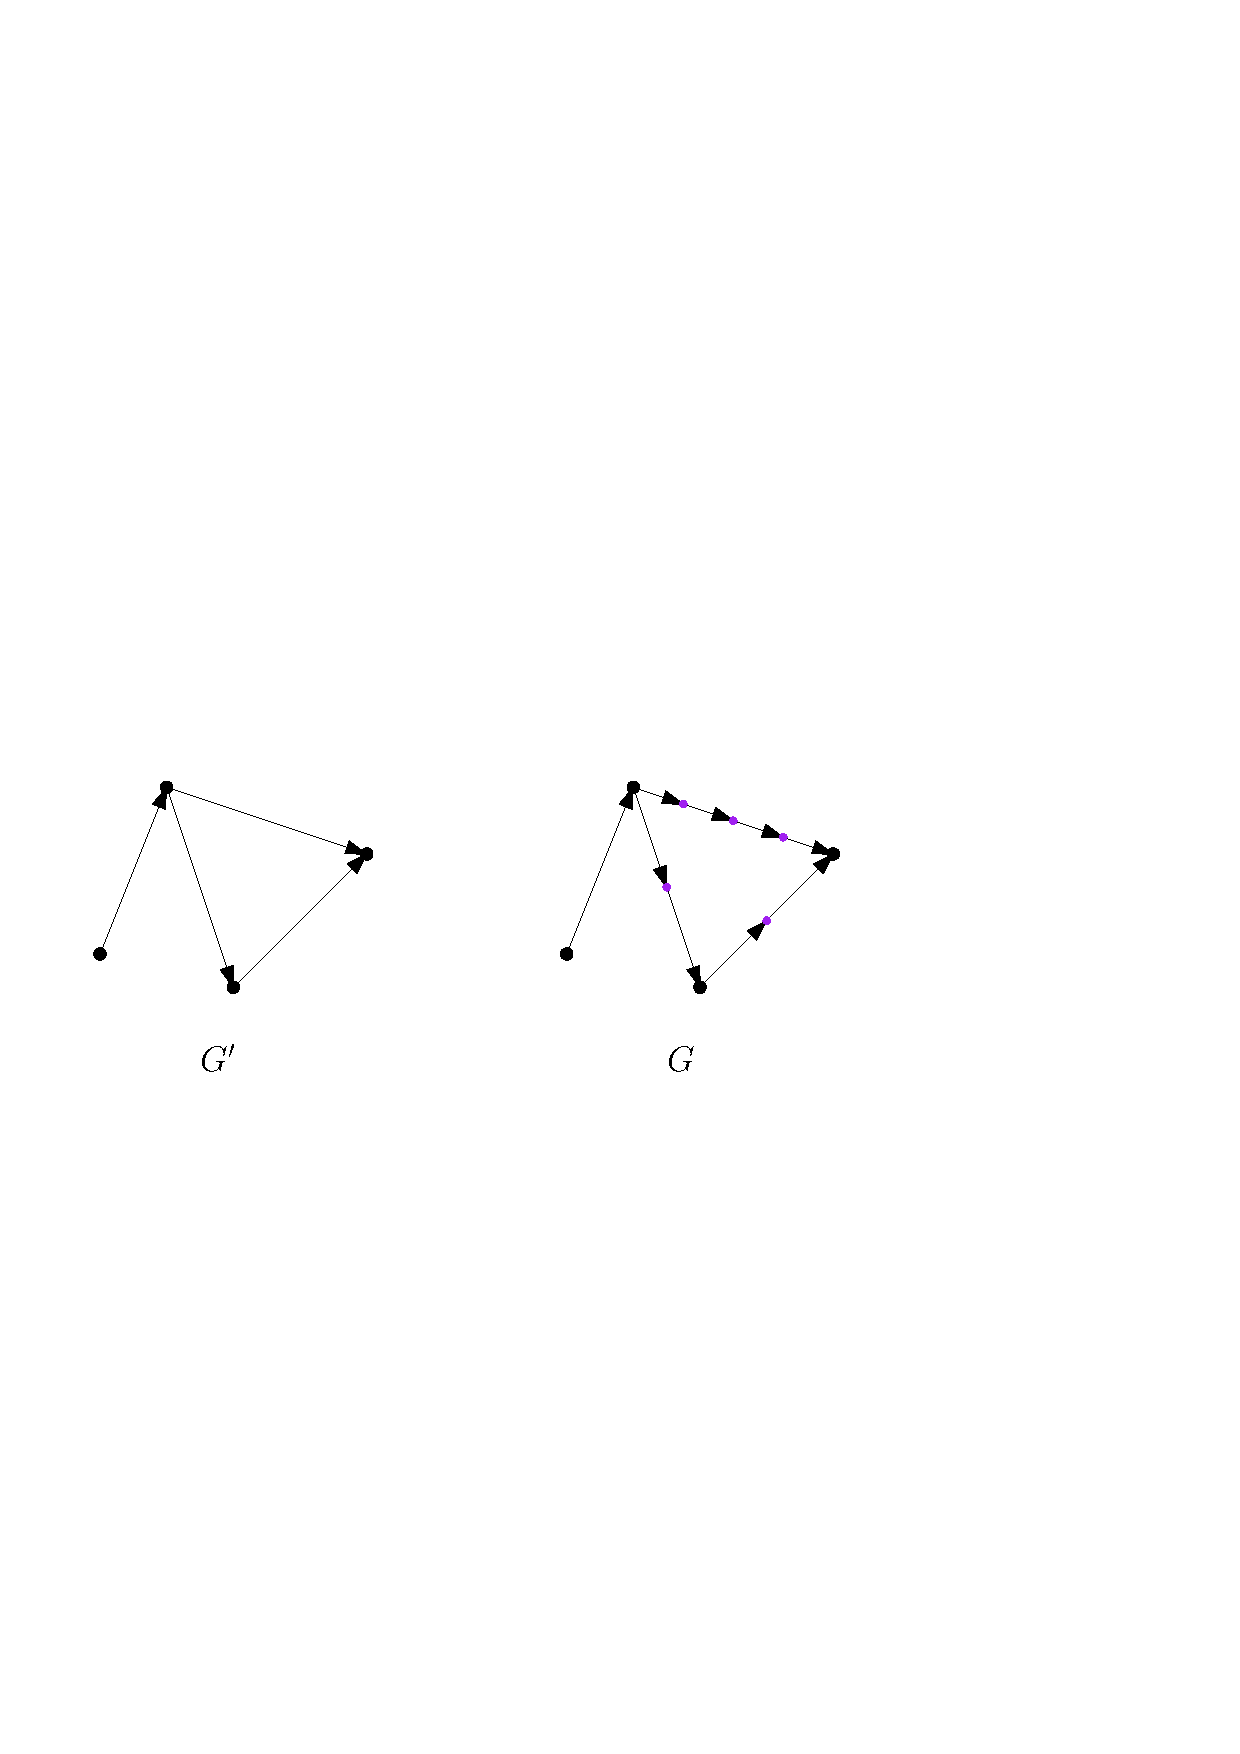
\includegraphics[scale=0.6]{./pictures/long_edges_example.pdf}
	\end{center}

	Хотим записать на ребре $G'$, например, цвет, или номер вершины, или номер ребра, и т.д.

\end{frame}

\begin{frame}{Результаты: Техника длинных ребер}
	\begin{theor}\label{theorem}
		Пусть есть алгоритм для задачи all-pairs CFL reachability с временной сложностью $\mathcal{O}(n^c \cdot poly(|G|)) = \mathcal{O}(n^c)$. Тогда существует алгоритм для задачи all-pairs CFL reachability на графах с длинными ребрами длины $k = o(\log n)$ с временной сложностью $\mathcal{O}(n^{c+c'}), \forall c' > 0$.
	\end{theor}
	
	\begin{theor}
		Если аналогичная теорема верна для графов с ребрами длины $k = \Omega(\log n)$, то верно хотя бы одно из следующих утверждений:
		
		 \begin{itemize}
		 	\item В сведении используется граф, структура которого "сильно отличается"$\,$ от входного графа
		 	\item Обе гипотезы APSP и 3SUM неверны. 
		 \end{itemize}
	\end{theor}
\end{frame}
	
\begin{frame}{Итог}
	\begin{itemize}
		\item Получены новые сведения к задаче CFL reachability и близким к ней задачам.
		\item Доказана лучшая оценка на сложность задачи CFL reachability для случая путей ограниченной длины.
		\item  Рассмотрена техника длинных ребер: ее возможности и ограничения.
	\end{itemize}
\end{frame}

\begin{frame}
	\begin{center}	
		\Large{Спасибо за внимание!}
	\end{center}
\end{frame}


\end{document}